\documentclass[11pt]{article}
\usepackage{graphicx}
\usepackage{amssymb}
\usepackage{epstopdf}
\usepackage{rotating}
\usepackage{amsfonts}
\usepackage{natbib}
\usepackage{subfigure}
\usepackage{pdfsync}
\usepackage{xspace}
\usepackage{color}
\usepackage{url}
\usepackage{nameref}
%\usepackage[pdftex, colorlinks=true,urlcolor=blue]{hyperref}
%\usepackage{wallpaper}

%%%% HERE IS SOME WATERMARK STUFF
%\addtolength{\wpXoffset}{-.2in}
%\CenterWallPaper{1.1}{/Users/eriq/Documents/work/nonprj/WaterMarks/StrictDraftWatermark.eps}


\DeclareGraphicsRule{.tif}{png}{.png}{`convert #1 `dirname #1`/`basename #1 .tif`.png}

%% My baseurl.  Can be changed as necessary.


%% some handy things for making bold math
\def\bm#1{\mathpalette\bmstyle{#1}}
\def\bmstyle#1#2{\mbox{\boldmath$#1#2$}}
\newcommand{\thh}{^\mathrm{th}}


%% Some pretty etc.'s, etc...
\newcommand{\cf}{{\em cf.}\xspace }
\newcommand{\eg}{{\em e.g.},\xspace }
\newcommand{\ie}{{\em i.e.},\xspace }
\newcommand{\etal}{{\em et al.}\ }
\newcommand{\etc}{{\em etc.}\@\xspace}


\newcommand{\CR}{\mathrm{CR}}
\newcommand{\CWT}{\mathrm{CWT}}
\newcommand{\PBT}{\mathrm{PBT}}
\newcommand{\Var}{\mathrm{Var}}
\newcommand{\btheta}{\bm{\theta}}

%% the page dimensions from TeXShop's default---very nice
\textwidth = 6.5 in
\textheight = 9 in
\oddsidemargin = 0.0 in
\evensidemargin = 0.0 in
\topmargin = 0.0 in
\headheight = 0.0 in
\headsep = 0.0 in
\parskip = 0.2in
\parindent = 0.0in


\title{Assessing the potential for PBT to deliver \\
estimates currently obtained using CWTs: \\
a data-driven, large scale assessment}
\author{Eric C. Anderson\thanks{
    Fisheries Ecology Division, 
    Southwest Fisheries Science Center, 
    110 Shaffer Road,
    Santa Cruz, CA 95060}
}
\begin{document}

\maketitle

\tableofcontents

\section{Introduction}
Here, we seek to address this information need:
\begin{quote}
{\sl Assessment of the degree to which this system could or could not deliver estimates of the key life history and fishery parameters that are currently delivered from the CWT program and do so with similar or better accuracy (i.e., consider errors of estimation). Identify areas or issues where implementation of PBT on a coast-wide basis seems most problematic. }
\end{quote}

There are two main variables that influence the accuracy of different estimates of life-history and 
fishery parameters obtained from CWT or PBT data: 1) the number of tags (CWT-based or PBT-based) that 
are actually recovered, and 2) the accuracy with which those tags can be expanded to meaningful estimates
of the expanded number of recoveries.  The main factor driving (2) is the accuracy with
which the tagging rate is known.  We deal with (2) in a separate document, ``Variation in
Parentage-Based Tagging and Coded-Wire  Tagging  Rates.''  In this document, we treat issue (1), assessing
the degree to which increasing tagging rates by using  PBT can improve
tag-recovery rates.  

Because tagging a higher fraction of any stock can be done cheaply with PBT, it is tempting to
think that increasing tagging rates using PBT will invariably lead to higher recovery rates
for all the release groups.  This is, however, untrue: it is necessary to mark (ad-clip) PBT-tagged
fish in order to recover them, and indiscriminately increasing the mark rate on numerous stocks
will almost certainly reduce the fraction of marked fish (in mixed fisheries) that originate from
certain weak or underrepresented stocks, decreasing the recovery rate for those stocks.  Therefore, 
increasing tag rates through PBT must be done in a more nuanced and selective fashion.  

The degree to which selective increases in tagging rates can improve recovery rates for many 
stocks depends on a number of factors.  For example, recovery rates for a weak stock cannot be 
easily increased if that stock is already tagged at 100\%.  Furthermore,
the effect upon any particular fishery of increasing the tagging rates on a group of stocks depends
fundamentally upon the relative composition of those stocks in the fishery.  And, of course,
tag-rate increases that improve recoveries of a release group that is rare in one fishery might,
if that stock is common in a second fishery, have the effect of reducing recovery rates of other
stocks in that second fishery.  On top of that, the effect of increasing tag rates on a fishery will
depend on other features of the fishery, for example, whether it is visually or electronically sampled.
Therefore, the potential for PBT to deliver improved estimates of fishery parameters on a coastwide scale
can only be answered by taking account of the stock composition of those fisheries and the sampling
schemes employed in them.  

Here, we divide the marine fisheries in the year 2012 for Chinook salmon along
the Pacific Coast of North America into
18 regions and estimate the composition of fish recovered from those regions by applying a novel
Bayesian estimation model to data from the Regional Mark Information System (RMIS) data base.  After
confirming that the model fits the data well, we use the estimated composition of release groups
in each region to explore how expected recovery rates change under different scenarios of modifying the 
tagging and marking rates of PBT.  The expected recovery rates of PBT-tagged fish can be easily compared
to the expected recovery rates of CWTs given current tagging and marking rates, which provides a principled
way of assessing the degree to which a PBT program might be able to yield more recoveries, 
and hence more accurate estimates, from multiple release groups across the whole coast.   


The remainder of this document is divided into five main sections.  In {\sc \nameref{sec:prelims}},
we summarize and make explicit some of the assumptions and operating perspectives we have adopted
in this work.  {\sc \nameref{sec:bayes}} gives details of the model used to estimate
proportions of different release groups in fisheries.  {\sc \nameref{sec:agg}} describes how we divided
Chinook fisheries in 2012 into a few large recovery areas and summarizes the number of CWTs from
each release group recovered in those fisheries. In {\sc \nameref{sec:estimation}} we apply the
Bayesian model to each large recovery area and present the estimates, as well as the posterior
predictive checks which verify that the model fits the data.  Finally, in
{\sc\nameref{sec:compare}}, we discuss different schemes for setting tagging rates at
PBT hatcheries and then compare expected recovery rates under those schemes to the recovery
rates expected from using current CWT tagging rates.  





\section{Preliminaries and Assumptions \label{sec:prelims}}

In order to make this undertaking manageable, while still yielding useful information, I make
a few assumptions, listed below:
\begin{enumerate}
\item {\sl The tag-code is the basic unit for fishery estimation.} I suspect that for many estimation purposes
it is customary to aggregate multiple tag-codes (release groups) from a given hatchery or across multiple
hatcheries in a single stock, but I have not done that here.  Our guidance has included the fact that a 
PBT system must accommodate multiple release groups within any hatchery, so
there seems a good precedent for focusing on tag-codes as the basic unit for estimation.
\item {\sl Fishery samples across nearby locations and over time can be aggregated. } Here I am basically assuming
that the composition of fisheries across nearby locations and over a year can be regarded as identical.  This is
necessary because very few fishery strata contain enough coded wire tag recoveries to yield a reliable estimate
of the proportion of fish from each release group in the fishery. {\bf It would be very helpful if the technical
advisory committee were able to provide a list of how
different agencies aggregate fishery location and time strata for their management purposes}.
Not knowing that myself, I have just agglomerated spatially
proximate fishery locations over entire years to achieve samples of 500 or more CWTs.  Obviously, this is 
flexible and could be changed with input from the committee.   While this will not
reflect compositional changes over seasons, my feeling is
that we are after a reasonable approximation of what the true composition is, and this will likely
suffice.
\item {\sl The tagged and marked fractions of a release group are constant over the life of the fish.}  This
assumption would be violated if marked or tagged fish experience higher mortality than their unmarked
counterparts, as could be the case in the presence of very strong mark-selective fishing pressure.  Dealing with
that seems like it would be overkill for these simulations.  Remember, we are interested in getting results
for fisheries with proportions that might reasonably be encountered, and I hope that the occurrence of
some extra mortality on tagged fish will not render the proportions used in the simulation ``unreasonable.''
\item {\sl The only type of mark we concern ourselves with in the estimation of proportions is the
adipose clip.}  An adipose clip in conjunction with another mark is just counted simply as an ad-clip.
\item {\sl Currently I am not addressing suitability of either PBT or CWTs for doing DIT-based estimation.}
\item {\sl This is being developed at the moment for recoveries from fisheries, but it could easily be extended to
escapement, \etc}
\end{enumerate}


\section{Bayesian Estimation of Release Group Proportions \label{sec:bayes}}

We propose a simple model to estimate the composition of fish from different release groups
from CWT recovery data.  We then specify a Gibbs sampler to sample from the posterior
distribution of the parameters in the model.

\subsection{Parameters}

Let $\theta_g$ be
the probability that a fish sampled 
from the ocean within a given recovery area  is from release group $g$, $g = 1,\ldots, G$,
where $G$ is the total number of distinct tag codes with at least one recovery, coastwide,
during the year.  Denote all of those probabilities by $\btheta = (\theta_1, \ldots, \theta_G)$.
We don't specifically denote the recovery area in order to avoid an
overproliferation of subscripts, but remind the reader that recovery $\theta_g$ is defined in
reference to a particular recovery area. Note that $\btheta$ might not reflect the
true composition of fish in the recovery area because of length restrictions on the catch, \etc  We contend
that this is not a great concern because, for our purpose, what we wish to estimate is the
probability that a fish from a certain release group will
be caught and retained in the fishery, and that is what precisely what $\theta_g$ reflects.


We define each release group, $g$, to corresond explicitly to a tag code; however, it is important
to understand that $\theta_g$ refers not just to the fraction of fish from release group $g$ that
have CWTs, but {\em all} of the fish in the release group $g$, whether they have
a CWT or not. As stated above, 
will think of tag codes, $g$, as being indexed from 1 up to $G$ for the $G$ possible tag codes
that were actually observed in some marine fishery along the coast during the given year. 


We include several other categories:
\begin{description}
\item{$A+$ and $A-$:}~~Fish from non-associated release groups that carry agency only or blank wire.  These fish cannot be identified to release group but they do all carry wire. The $+$ and the $-$ refer to whether or
not the fish is ad-clipped.
\item{$U+$ and $U-$:}~~Fish that don't carry wire of any sort and are not part of an associated release group.  If
they have an ad-clip, they are part of $U+$; if they don't, they are part of $U-$.  Untagged and unmarked wild
fish are part of $U-$, as are unmarked fish from non-associated releases.  Untagged but marked fish from
non-associated releases are in $U+$.
\end{description}
Some portions of the $A$ and $U$ categories are not likely to be easily estimated, as they represent the ``leftover'' after all
the fish from associated releases are accounted for.  It will be interesting to see how their inclusion affects
estimates of composition uncertainty. The parameter we are interested in is thus $\btheta = (\theta_1,\ldots,\theta_{G},
\theta_{A+}, \theta_{A-}, \theta_{U+}, \theta_{U-})$, and we note that 
\[
\theta_{A+} + \theta_{A-} + \theta_{U+} + \theta_{U-} + \sum_{g=1}^{G} \theta_g = 1.
\] 


Each tagged release group $g$ is assumed to have a marked fraction, $f^{(m)}_g$ and an unmarked fraction, $f^{(u)}_g$, 
such that $0 \leq f^{(m)}_g, f^{(u)}_g \leq 1$ and $f^{(m)}_g + f^{(u)}_g = 1$.  We consider a fish to be ``marked'' if it has an ad-clip (whether or
not in combination with another mark).   Associated with each of these fractions is a CWT tagging rate, $p$.  So, $p^{(m)}_g$ denotes the
fraction of the marked fish from release group $g$ that carry CWTs, and $p^{(u)}_g$ denotes the fraction
of unmarked fish from release group $g$ that carry CWTs; $0 \leq p^{(m)}_g, p^{(u)}_g \leq 1$;
however $p^{(m)}_g + p^{(u)}_g$ is not necessarily equal to 1.  For each $g=1,\ldots,G$, the values of the $p$'s and $f$'s can be obtained
from information stored in the RMIS release data base.


It is important to understand that I will be agglomerating different fishery strata in order to obtain
relatively large samples of CWTs with which to estimate $\btheta$.  In such cases I will assume that
$\btheta$ is identical across all agglomerated strata.  This is obviously a simplification, but it does not make 
sense to estimate a separate $\btheta$ for every stratum, some of which have only a few CWT recoveries.
The other consequence
of this policy is that I will likely end up using both visually and electronically detected samples, together, to 
estimate any particular $\btheta$.  Thus, we would like our estimation method to
appropriately weight information from each type of sample.  I believe the Bayesian framework I
describe below achieves that.

\subsection{Missing data formulation}
We can develop our estimation framework by noticing that we are missing information here
that would make the estimation problem quite easy---namely, if we knew the release group of every
fish we sampled in a fishery (whether it had a CWT or an ad-clip or not).  In that case, we would have a simple multinomial
formulation with a Dirichlet prior.  Of course, we don't know the release group of every sampled
fish---that is missing!  But thinking about the problem this way shows us that it is a classic
missing-data problem for which the EM-algorithm or Gibbs sampling are useful.  In our case we will
formulate a way to sample over the unknown origins of all of the sampled fish in a stratum (whether or 
not they have an ad-clip or carry a CWT) given 
everything else we know about them.
In other words, for every fish that is handled in some way (either visually inspected for an ad-clip or
electronically scanned for a CWT) we can sample over that crucial piece of missing data---the fish's origin.
Having sampled all the fish's tag-codes of origin we can use them to update our estimate of
$\btheta$---a simple Gibbs sampler that will be described in detail below.

\subsection{The data (missing and otherwise) for each ``sampled'' fish}

For each fish that is sampled---any fish that someone looks at to see if it has a mark, or
runs  through a metal detector to see if it beeps---the list below shows what we shall keep track of (and
update/impute as necessary).  The names in {\tt monospaced} font below refer to the specifications that
will be used in the computer code that goes with this project, and the mathematical notations immediately
following give
the indicator variables and their values that will be used in the upcoming mathematical formulations.
\begin{description}
	\item [{\tt detection\_method}:] ~~~$\delta_i^{(\mathrm{dm})}$~~~The method used to screen fish to discover CWTs. ($\delta_i^{(\mathrm{dm})}$ is the detection method of fish $i$ in the sample).
	\begin{itemize}
		\item [{\tt V}:] ~~~$\delta_i^{(\mathrm{dm})} = \mathrm{V}$~~~if the fish was visually sampled.
		\item [{\tt E}:] ~~~$\delta_i^{(\mathrm{dm})} = \mathrm{E}$~~~if the fish was electronically sampled.
	\end{itemize}
	\item [{\tt beep}:] ~~~$\delta_i^{(\mathrm{b})}$~~~Whether or not it beeped upon electronic detection. Possible values are:
	\begin{description}
		\item [{\tt yes}:] ~~~$\delta_i^{(\mathrm{b})} = 1$~~~The fish beeped when detected electronically.
		\item [{\tt no}:]  ~~~$\delta_i^{(\mathrm{b})} = 0$~~~The fish did not beep when detected electronically.
		\item [{\tt irrelevant}:] The fish was not sampled electronically.
		Must be irrelevant if detection\_method is {\tt V}. Might be irrelevant if the fish is part of a
		mark sample that is drawn {\em independently} of the beep-status for fish in a fishery with
		electronic detection.
	\end{description}
	\item [{\tt ad\_clipped}:]  ~~~$\delta_i^{(\mathrm{ac})}$~~~Does the fish have an adipose clip? 	An ad-clip, even in combination with any other marks is still counted.
	\begin{description}
		\item [{\tt yes}:]  ~~~$\delta_i^{(\mathrm{ac})} = 1$~~~The fish was observed to have an ad-clip.
		\item [{\tt no}:]  ~~~$\delta_i^{(\mathrm{ac})} = 0$~~~The fish was observed to {\em not} have an ad-clip.
		\item [\textcolor{blue}{{\tt unknown}}:]  ~~~$\delta_i^{(\mathrm{ac})} = \mbox{?}$~~~The fish was either not
		inspected for a mark, or it was and its mark status was ambiguous.
	\end{description}
	\item [{\tt cwt\_status}:] ~~~$\delta_i^{(\mathrm{cs})}$~~~Does the individual carry a CWT or not, and what category of wire is
	it? (this is {\em not} the same as the tag code of the fish).
	\begin{description}
		\item [{\tt cwt}:] ~~~$\delta_i^{(\mathrm{cs})} = 1$~~~The fish is known to carry a coded wire tag, and it
		was read appropriately.
		\item [{\tt no\_read}] ~~~$\delta_i^{(\mathrm{cs})} = n$~~~This corresponds to all fish that
		are observed to have a non-agency-only CWT but which is not readable, or was apparently read incorrectly.  This 
		includes the categories ``Tag lost before read,'' ``Tag not readable,'' 
		and ``Unresolved discrepancy.''
		\item [{\tt awt}:] ~~~$\delta_i^{(\mathrm{cs})} = a$~~~Agency-only or blank wire.
		\item [{\tt no\_tag}:] ~~~$\delta_i^{(\mathrm{cs})} = 0$~~~The fish is observed to {\em not} carry a CWT
		\item [\textcolor{blue}{{\tt unknown}}:] ~~~$\delta_i^{(\mathrm{cs})} = \mbox{?}$~~~It is unknown if the fish carried a CWT or not.  This would be the case, for example
		in fish that had an ad-clip but were not assessed for the presence of a CWT, or fish that did not have
		an ad-clip and were not assessed for the presence of a CWT.
	\end{description}
	\item [{\tt tag\_code}:] ~~~$\delta_i^{(\mathrm{tc})}$~~~What is the tag code that corresponds to the release group that the fish comes from.
	\begin{description}
		\item [{\tt code}:] ~~~$\delta_i^{(\mathrm{tc})} = g$~~~Whatever the tag code is for the release group the fish was a part of.  In fish without CWTs, this value will not be directly known, but we can still think of each
		fish as having an origin.
		use $g$ to index these tag codes.
		\item [\textcolor{blue}{{\tt unknown}}:] ~~~$\delta_i^{(\mathrm{tc})} = \mbox{?}$~~~This is the starting value
		for anything that is a {\tt no\_read}.
		\item [\textcolor{blue}{{\tt pending}}:] ~~~$\delta_i^{(\mathrm{tc})} = p$ ~~~~ This is the value we give things
		that have unknown cwt status.  
		\item [{\tt irrelevant}:] This is the case if {\tt cwt\_status} is not {\tt cwt}, {\tt no\_read}, or {\tt unknown}.  
	\end{description}
\end{description}


The states that constitute ``missing data'' or ``latent variables,'' and which may be updated
are colored blue.

\subsection{MCMC}

Given this setup, we can devise a straightforward Gibbs sampler that samples values of $\btheta$, and the 
{\tt unknown} variables for each sampled fish from their joint posterior distribution. To do so we will
introduce one more parameter whose value will be estimated from the data:  $\alpha$, the probability
of a false-positive beep.  $\alpha$ is the probability that a fish carrying no wire still gets a positive
beep during electronic detection.  We will assume that the false-negative rate for electronic detection is
negligible.

Sampling updated values for $\btheta$, given current values for the missing data is straightforward---the 
full conditional distribution for $\btheta$ is a Dirichlet distribution
with parameters equal to the prior weight on each
release group plus the number of fish from each release group.  Were we using this method to make actual estimates
for informing fishery management, it would probably make sense to spend a lot of time formulating a prior
for the tag codes that used information about proximity or similarity of different release groups. In our
case, however, since we merely want ``reasonable'' estimates for parameterizing a set of simulations, \textcolor{red}{I will assume
the prior on $\btheta$ is a Dirichlet distribution with overall weight determined to give roughly the correct
number of different tag codes (this can be derived from properties of the multivariate Ewens distribution.}

Given a current value for $\btheta$, the values of the {\tt unknown} variables, on all the sampled fish that have
{\tt unknown} values, can be simulated from their full conditional distribution.  For example,
consider a fish, $i$, that was visually-sampled, has an ad-clip, and had a CWT, but it was unreadable.  The 
probability that it is from a release group $g$ can be computed:
\[
P(\delta_i^{(\mathrm{tc})} = g | \delta_i^{(\mathrm{dm})}=\mathrm{V}, \delta_i^{(\mathrm{ac})} = 1, \delta_i^{(\mathrm{cs})} = 1)
\propto
\theta_g f_g^{(m)} p_g^{(m)}
\]
for all $g \in \{1,\ldots,G\}$. Computing this for every $g$ and normalizing it gives the full conditional distribution.

Imputing values for the missing data on fish that are not known to carry a CWT is a two step-process that follows
from decomposing the joint probability of their missing data into the product of two conditional probabilities.
To express this, it will be helpful to describe some marginal probabilities that can be computed from $\btheta$.  The marginal probability that a fish in the stratum has an ad-clip is:
\[
\phi^{(\mathrm{ac})} = \theta_{A+} + \theta_{U+} + \sum_{g=1}^G \theta_g f^{(m)}_g.
\]
The probability that a fish carries a coded wire tag associated with a release group, given it has an ad-clip is:
\[
\phi^{(\mathrm{cs}=1)}_1 =  \sum_{g=1}^G \theta_g f^{(m)}_g p^{(m)}_g,
\]
and given it does not have an ad-clip is:
\[
\phi^{(\mathrm{cs}=1)}_0 =  \sum_{g=1}^G \theta_g f^{(u)}_g p^{(u)}_g,
\]
\etc


\section{Aggregation and Characterization of 2012 Fisheries \label{sec:agg}}

\begin{sidewaysfigure}
\begin{center}
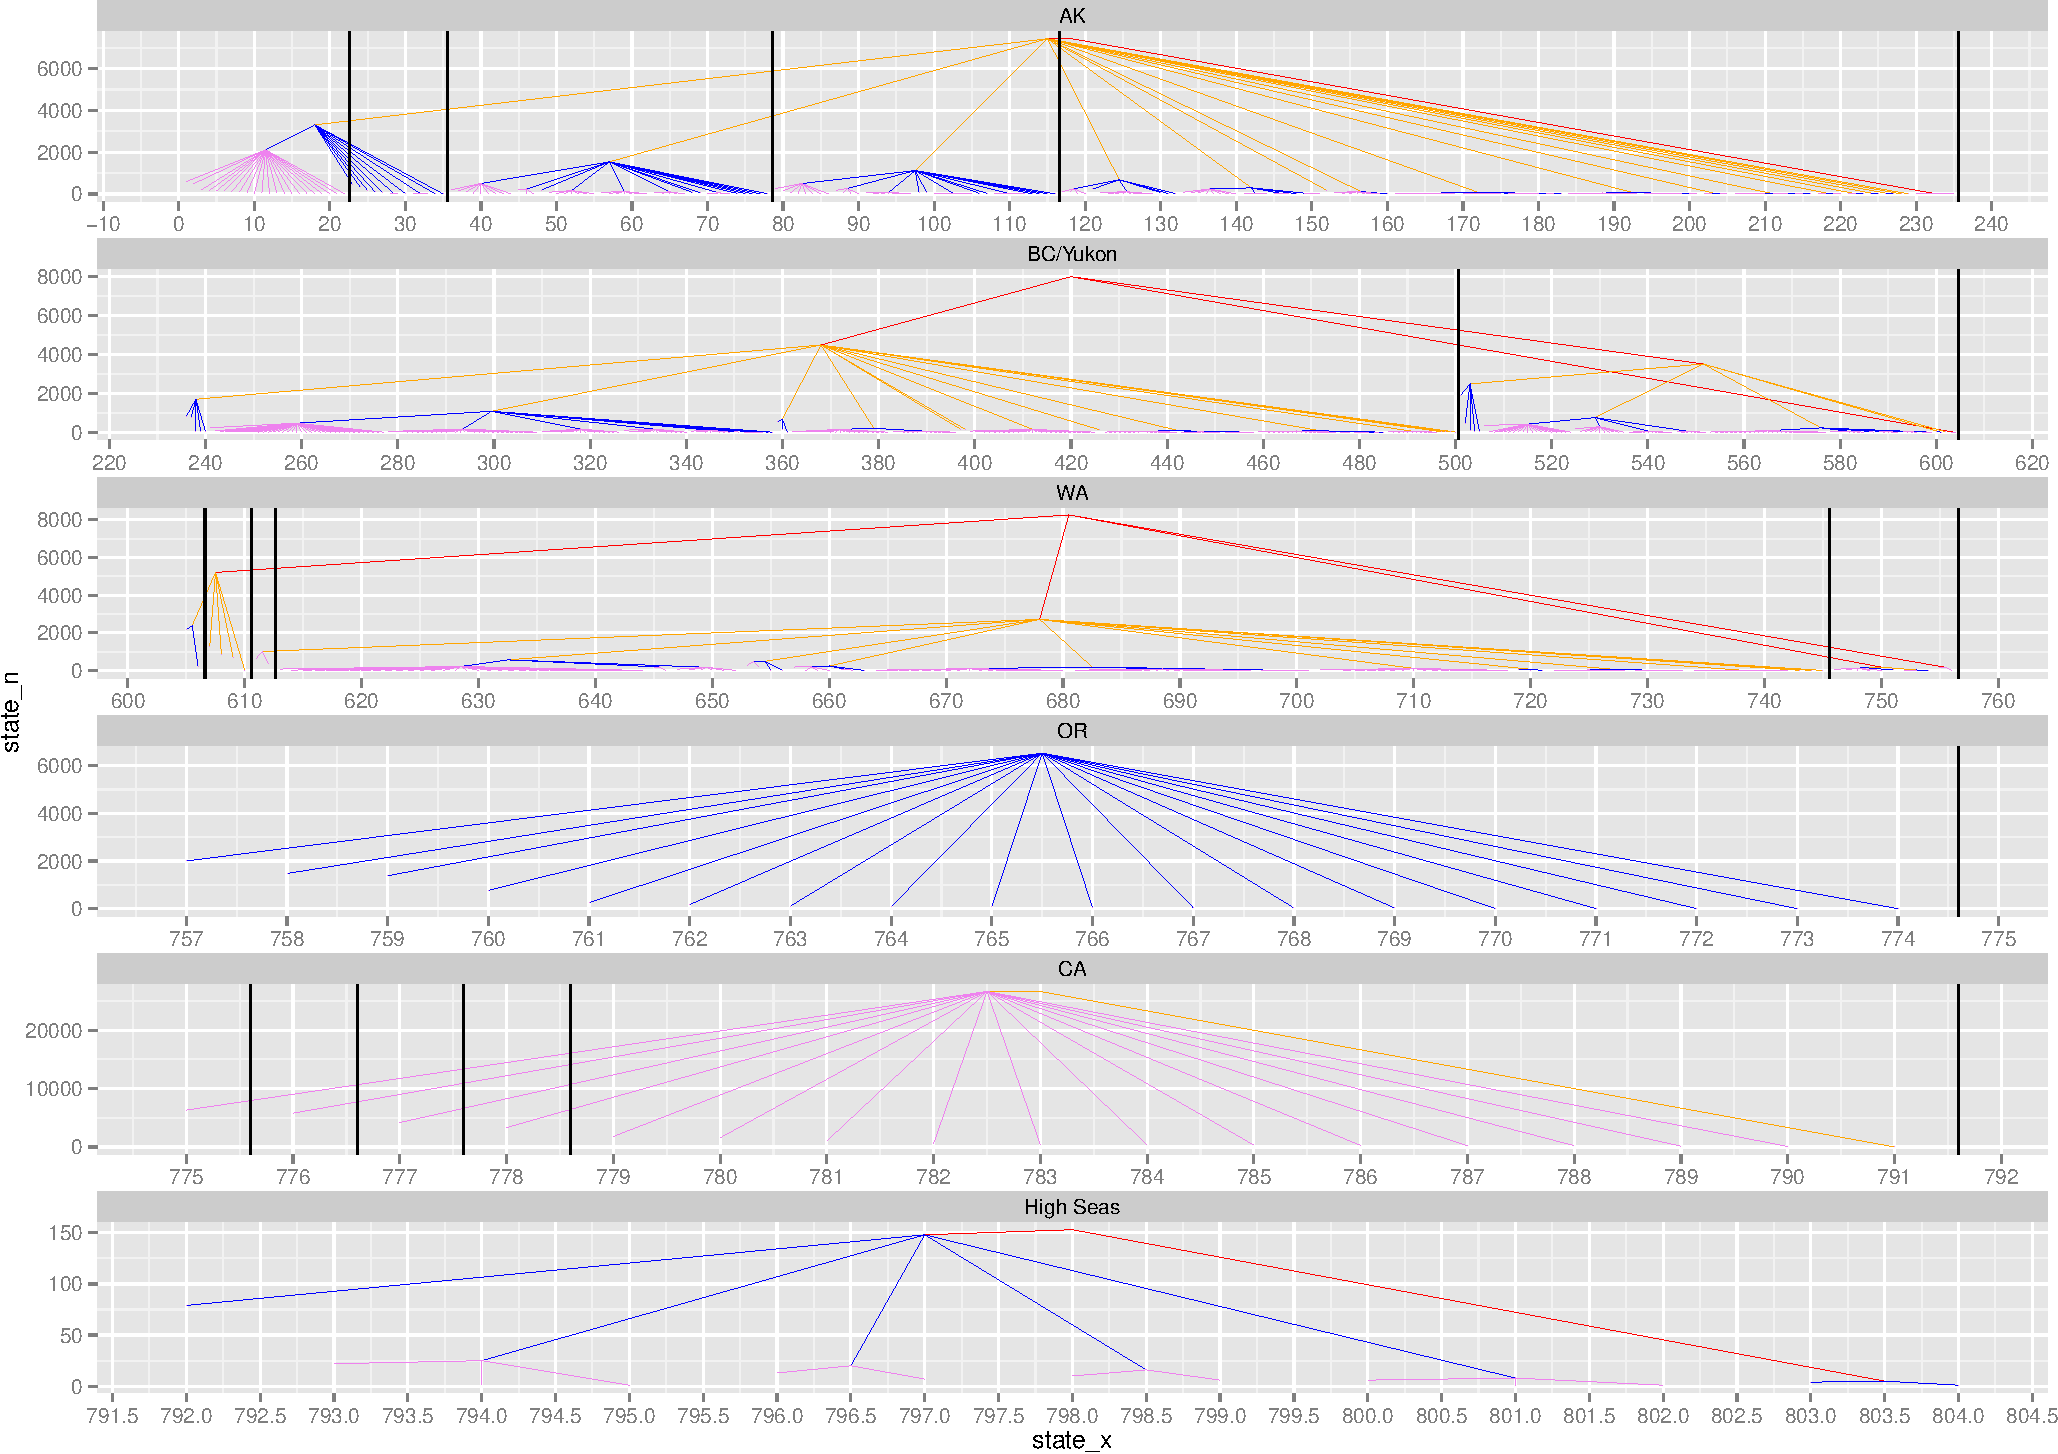
\includegraphics[width=\textwidth]{images/recovery_trees_divided.pdf}
\end{center}
\caption{Visual depiction of the hierarchical clustering of fishery recovery areas (and numbers of CWTs recovered)
in 2012.}
\end{sidewaysfigure}


\begin{sidewaysfigure}
\begin{center}
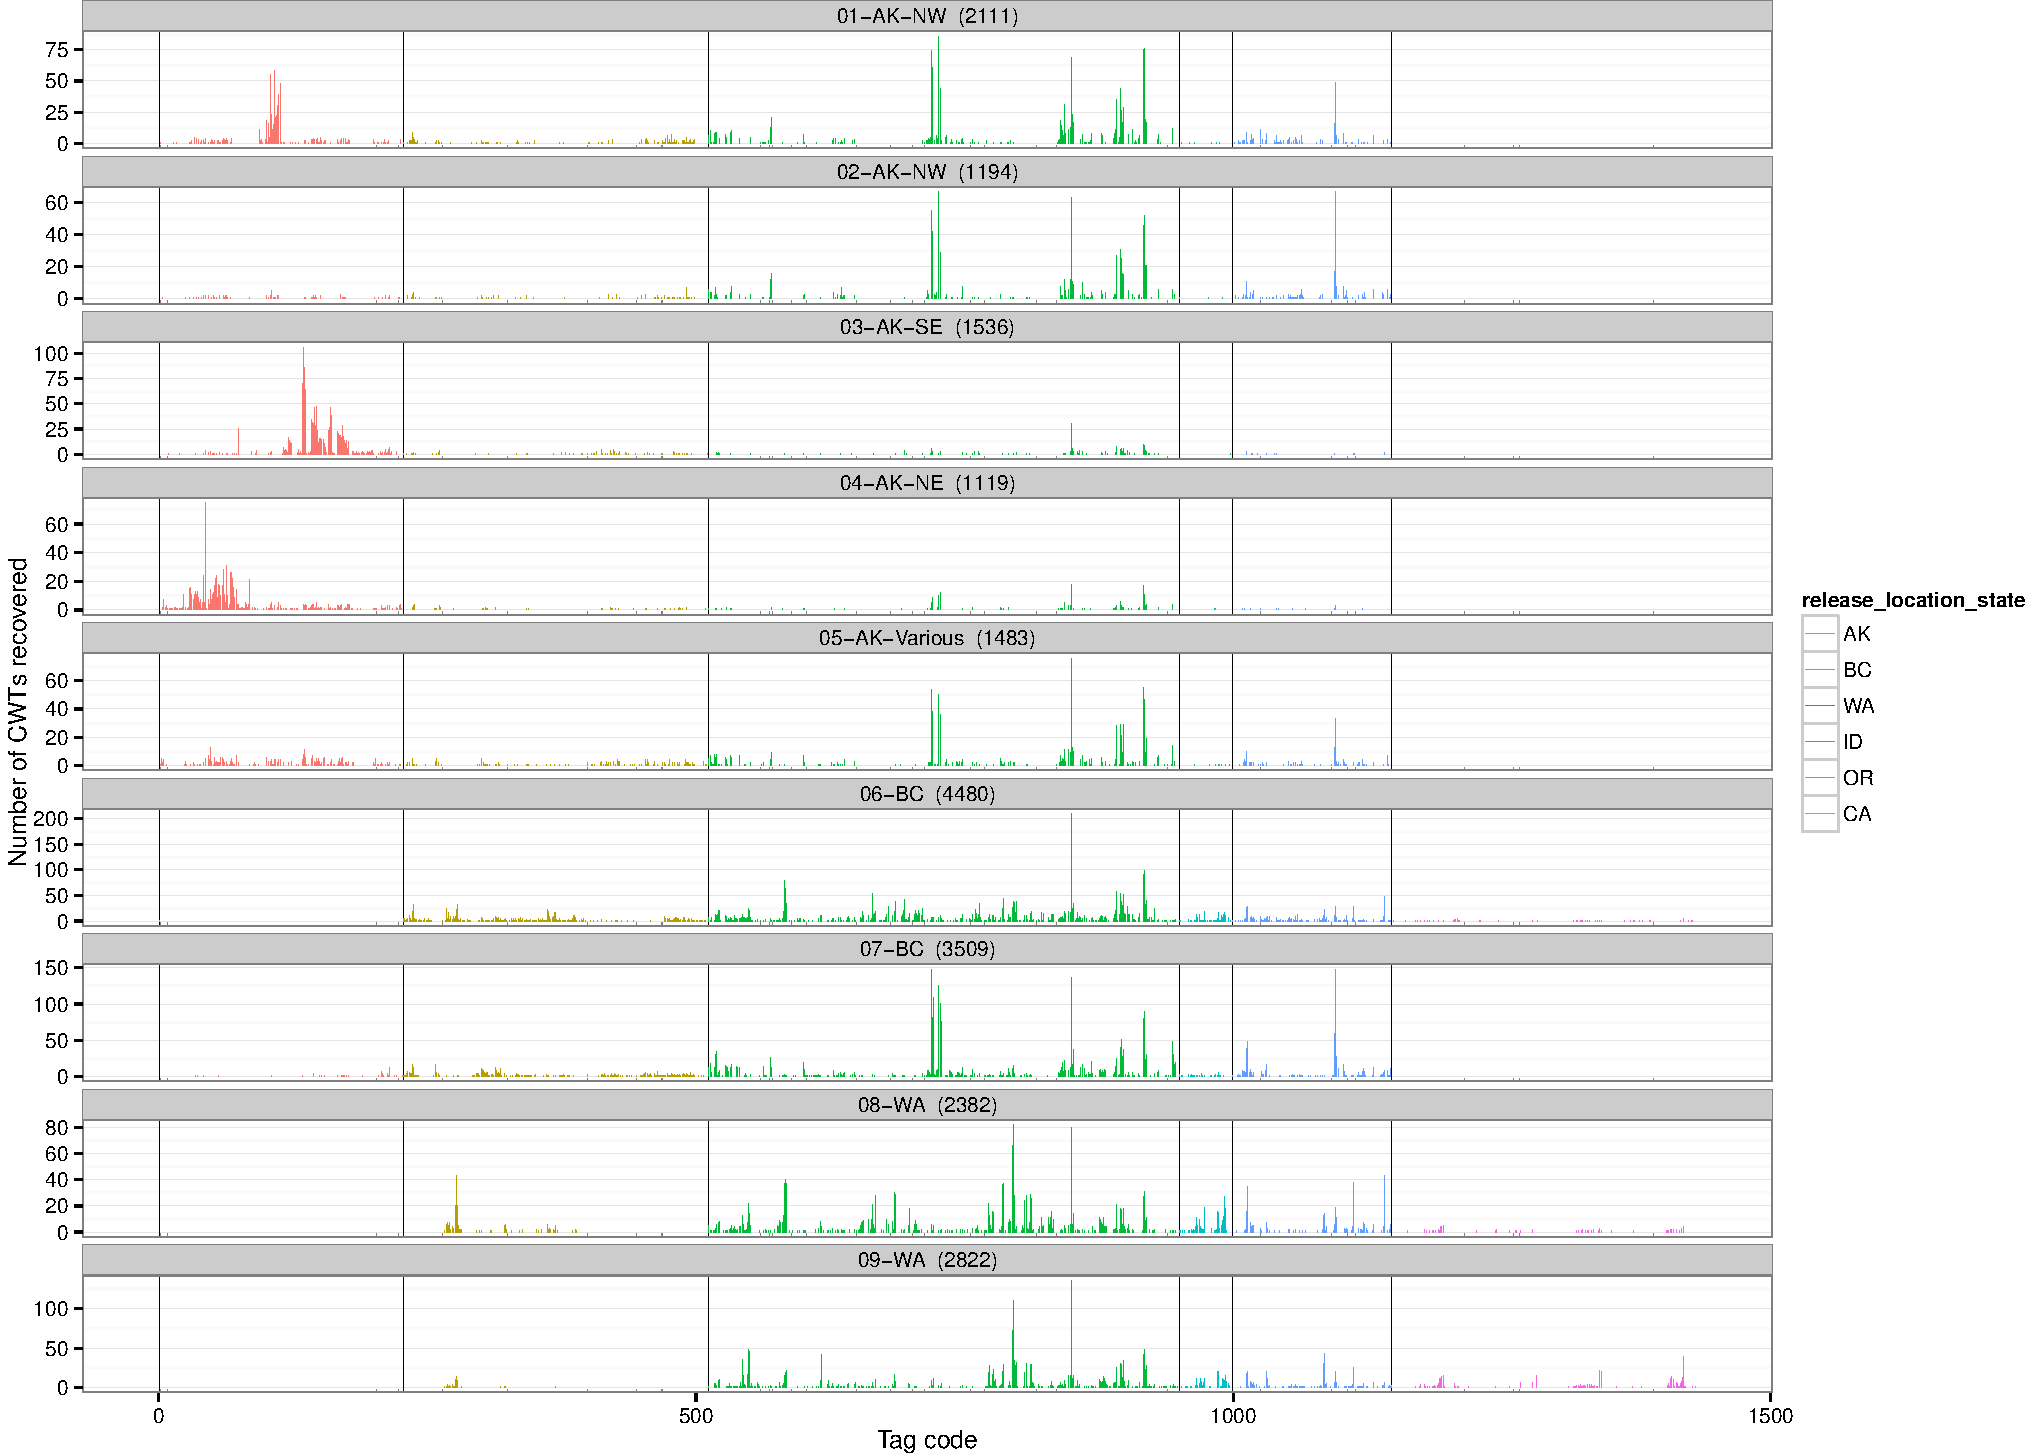
\includegraphics[width=\textwidth]{images/recovery_histo_panel_1.pdf}
\end{center}
\caption{The number of CWT recoveries from 1435 Chinook tag codes across different recovery areas in 2012, from Alaska to Washington.}
\end{sidewaysfigure}


\begin{sidewaysfigure}
\begin{center}
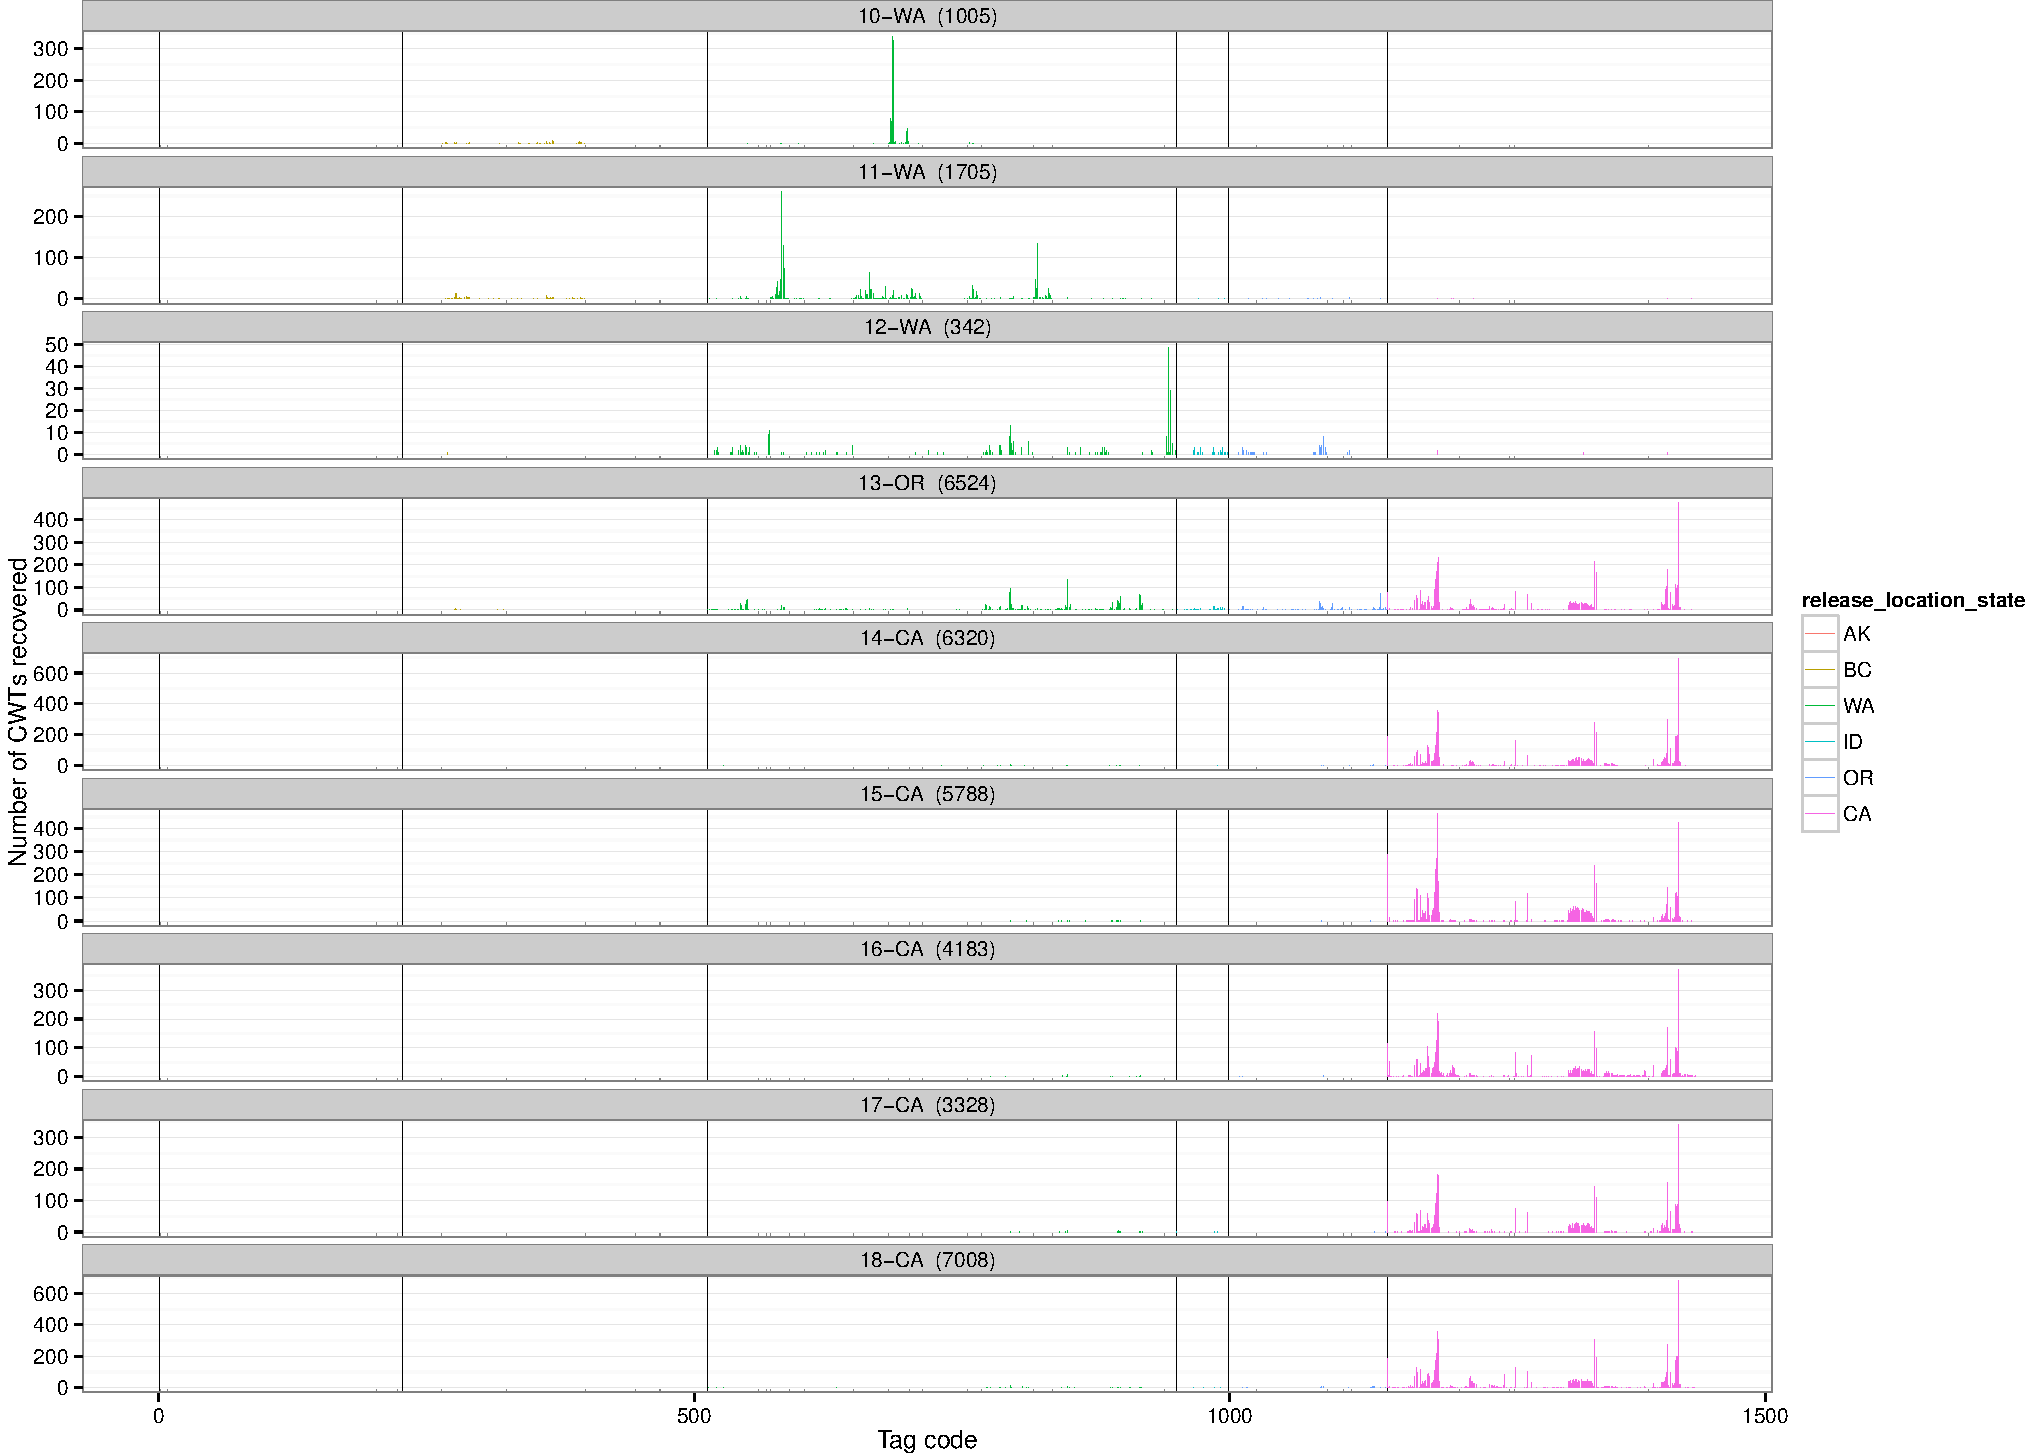
\includegraphics[width=\textwidth]{images/recovery_histo_panel_2.pdf}
\end{center}
\caption{The number of CWT recoveries from 1435 Chinook tag codes across different recovery areas in 2012, from Washington to California.}
\end{sidewaysfigure}


\section{Estimation of $\btheta$ in Fisheries Along the Coast \label{sec:estimation}}

\begin{sidewaysfigure}
\begin{center}
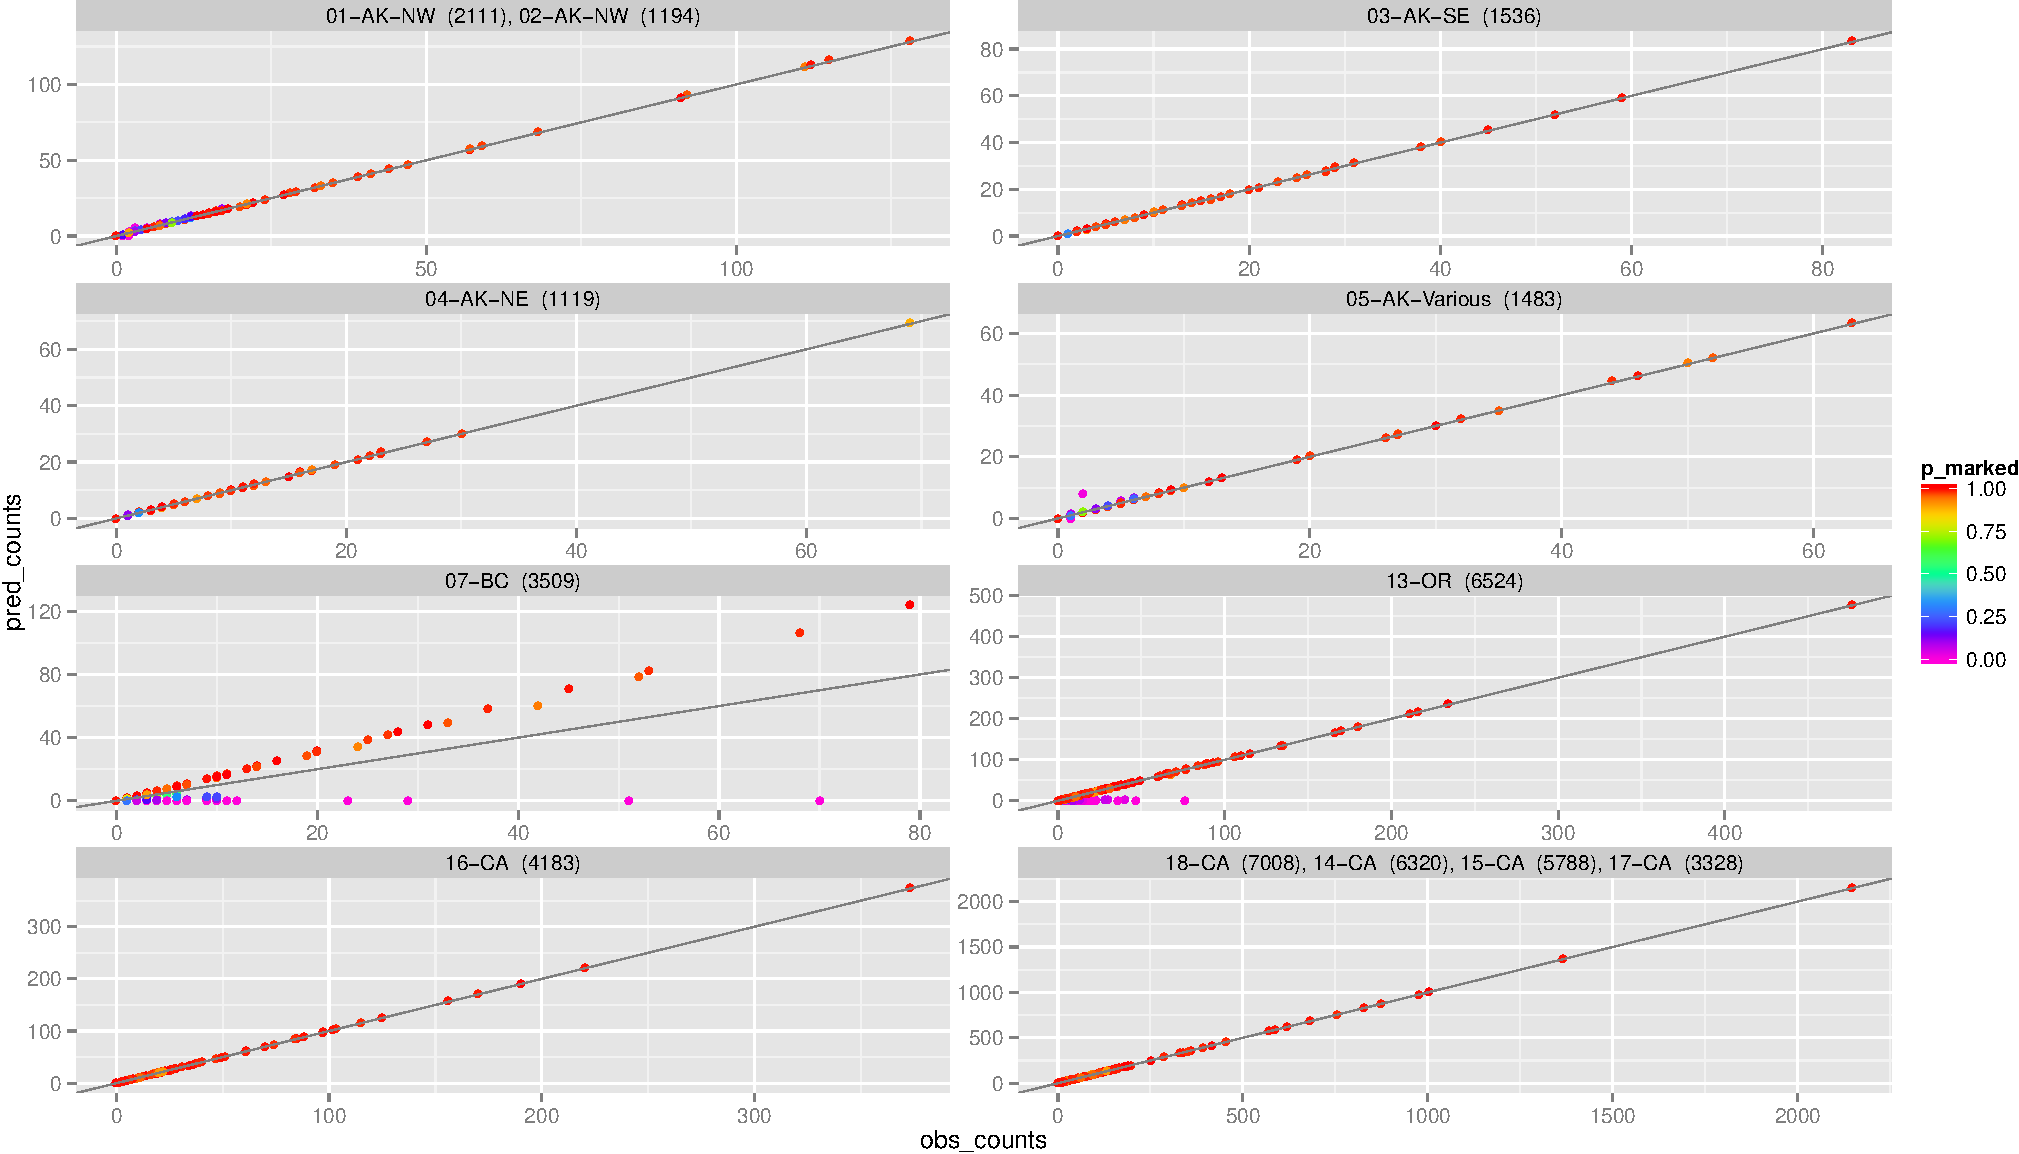
\includegraphics[width=\textwidth]{images/actual_vs_pred_cwt_recoveries_p_marked.pdf}
\end{center}
\caption{Posterior predictive checks of the the number of CWT recoveries predicted from the parameter estimates compared
to the actual number of recoveries.  Each point is a tag code which is colored according to $p_m$.  Note that occurrence
of BC release groups with $p_m$ reported to be 0.}
\end{sidewaysfigure}



\begin{sidewaysfigure}
\begin{center}
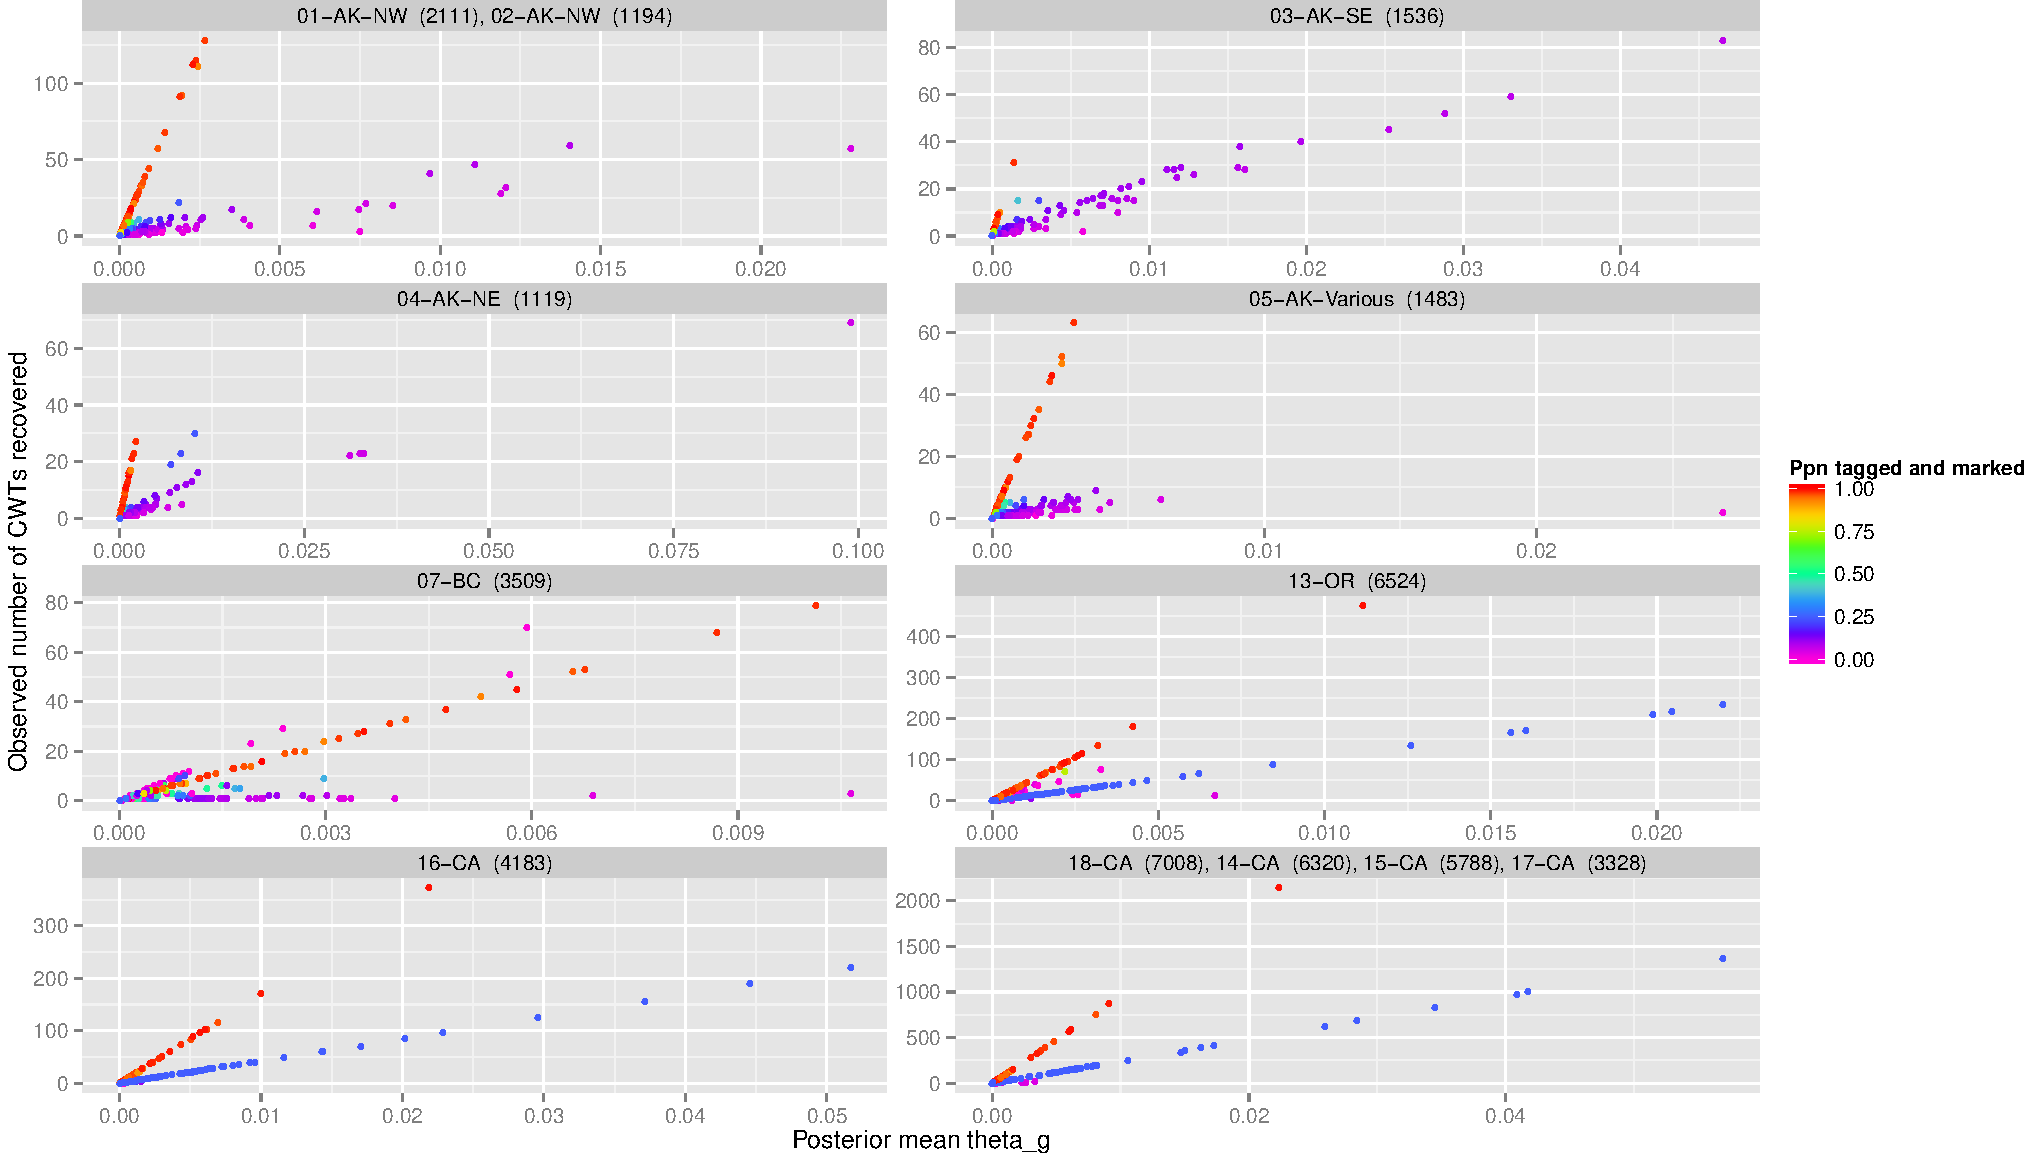
\includegraphics[width=\textwidth]{images/post_mean_theta_v_counts_f_marked_times_p_marked.pdf}
\end{center}
\caption{Posterior mean $\theta_g$ plotted on $x$-axis with observed number of CWTs recovered on $y$.  Each point is a
tag code colored by the proportion of the release group associated with the tag code that is both ad-clipped and tagged.}
\end{sidewaysfigure}



\section{Comparison of PBT to CWTs \label{sec:compare}}

Not yet done.

\bibliography{../bibstuff/pbtfeas}
\bibliographystyle{../bibstuff/men}
 \end{document}
